\subsubsection{\textit{Interfacing Input/Output}}
\textit{Interfacing I/O} adalah peralatan yang digunakan untuk menghubungkan suatu piranti dengan CPU melalui \textit{bus}. Tujuannya adalah mengontrol dan mentransfer data antara perangkat I/O dan CPU/memori melalui \textit{bus} dan \textit{controller}.
Komponen \textit{Interfacing I/O}:
\begin{itemize}
    \item Perangkat I/O: \textit{keyboard, mouse, monitor, printer,} dll.
    \item I/O \textit{Controller}: Perangkat keras yang mengontrol dan mengelola komunikasi antara 
    \item \textit{Bus}: Jalur komunikasi data antara perangkat I/O dan sistem komputer.
    \item \textit{Driver Software}: Perangkat lunak yang memungkinkan sistem operasi mengenali dan mengontrol perangkat I/O.
\end{itemize}

\subsubsection{Sistem Prosesor}
\begin{enumerate}
    \item {Saluran I/O}
Merupakan sebuah prosesor khusus dengan kemampuan terbatas yang disusun untuk interface beberapa piranti I/O ke memori. Saluran I/O dapat melakukan pendeteksian dan pembetulan kesaIahan dan beroperasi dalam basis \textit{cycle stealing}. Saluran I/O berkomunikasi dengan CPU sebagai suatu fasiIitas DMA dan berkomunikasi dengan piranti I/O seolah¬-olah sebuah CPU. Karena piranti I/O mempunyai kecepatan transfer yang berbeda-beda, maka saluran dibagi menjadi 3 pelayanan, yaitu:
\begin{enumerate}
    \item Saluran \textit{Multiplexer} \\
    Digunakan untuk menghubungkan piranti yang berkecepatan rendah dan sedang serta mengoperasikannya secara bersamaan dengan \textit{multiplexing}.
    \item  Saluran \textit{Selector} \\
    Digunakan untuk menghubungkan piranti I/O yang berkecepatan tinggi tanpa \textit{multiplexing}. Contoh: pita magnetis, \textit{disk}.
    \item Saluran \textit{Multiplexer} Blok \\
    Merupakan kombinasi dari dua pelayanan diatas.
\end{enumerate}
\end{enumerate}


\subsubsection{Prosesor I/O}
Merupakan komputer umum yang berkomunikasi dengan memori utama melalui fasilitas DMA system bus dan dengan piranti I/O atas satu atau lebih bus I/O.
Ada 2 mode yaitu:
\begin{enumerate}
    \item \textit{Single Shared bus} \\
    Setiap IOP mengendalikan sejumlah piranti I/O tertentu yang tetap.
\begin{figure}[h]
    \centering
    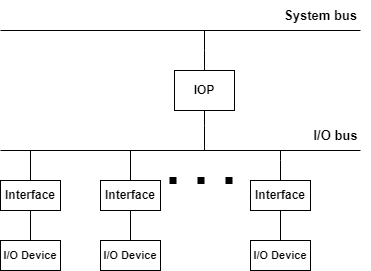
\includegraphics[width=0.5\textwidth]{/asset/Single.png}  % Sesuaikan nama file dan ukurannya
    \caption{Single Matrix bus}
    \label{fig:contoh_gambar}
\end{figure}
    \item \textit{Switching Matriks bus} \\
    Setiap IOP mengendalikan satu piranti I/O
    \begin{figure}[h]
    \centering
    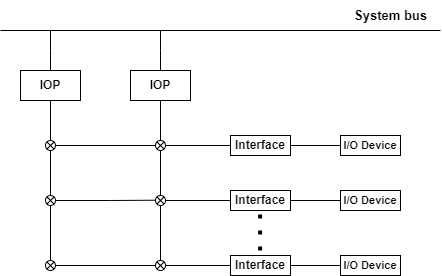
\includegraphics[width=0.5\textwidth]{/asset/Switching.png}  % Sesuaikan nama file dan ukurannya
    \caption{Switching Matriks bus}
    \label{fig:contoh_gambar}
\end{figure}
    \item Konfigurasi \textit{Multiprosesor} \\
    Di dalam satu komputer seakan-akan terdapat beberapa \textit{mikroprosesor}, meskipun sebenarnya \textit{mikroprosesor} utamanya hanya satu, sedangkan yang Iainnya berupa prosesor I/O (lOP). Hubungan yang paling sederhana menggunakan \textit{common bus}.
    \begin{figure}[h]
    \centering
    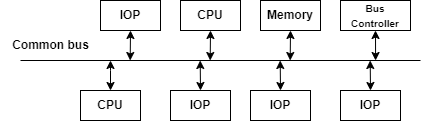
\includegraphics[width=0.5\textwidth]{/asset/Konfigurasi.png}  % Sesuaikan nama file dan ukurannya
    \caption{Ini adalah gambar contoh dari multithreading.}
    \label{fig:contoh_gambar}
\end{figure}
    \begin{itemize}
    \item \textit{Bus} umum bersifat membagi waktu (\textit{time shared}) oleh semua prosesor dan hanya satu prosesor yang dapat mengakses memori pada waktu tertentu.Tetapi dapat juga menggunakan \textit{bus} umum ke dalam organisasi \textit{multiprosesor dual bus}.
    \item Setiap komputer dihubungkan suatu pengendali sistem ke \textit{bus} umum.
    \item Komunikasi interkomputer ini dilakukan pada sistem \textit{bus} melalui memori umum.
\end{itemize}
\begin{figure}[h]
    \centering
    \includegraphics[width=0.5\textwidth]{/asset/systemBus.png}  % Sesuaikan nama file dan ukurannya
    \caption{System bus}
    \label{fig:contoh_gambar}
\end{figure}
\end{enumerate}